%
% Auteur initial inconnu.
% Modifié par olivier.ploton@univ-tours.fr le 21/09/2021
% À compiler avec pdflatex, bibilographie avec biber.
% Tous les fichiers doivent être encodés en UTF-8
% S'utilise en présence du fichier de bibiographie biblio.bib
% et des dossiers polytech/ (classe) et pic/ (images)
%

\documentclass{polytech/polytech}
\usepackage[strings]{underscore} % utile pour les _ dans la biblio (DOI)

% Fixe la présentation des listings
\lstset{
 columns=fixed,       
 numbers=left,                              
 numberstyle=\tiny\color{gray},             
 frame=single,                              
 backgroundcolor=\color[RGB]{255,255,255},  
 keywordstyle=\color[RGB]{40,40,255},       
 numberstyle=\footnotesize\color{darkgray}, 
 commentstyle=\it\color[RGB]{0,96,96},      
 stringstyle=\rmfamily\slshape\color[RGB]{128,0,0},  
 showstringspaces=false,                    
 language=C++
}

% Quelques formatages supplémentaires
\numberwithin{figure}{chapter}
\renewcommand\thesubsection{\thesection.\arabic{subsection}} 

% dossier des images
\graphicspath{{./pic/}}

%%%%%%%%%%%%%%%%%%%%%%%%%%%%%%%%%%%%%%%%

%
% Paramètres à fixer avant de commencer le document
%

\typereport{prddi5}       

\reportyear{2022-2023}

\title{Deep-Agora}
\subtitle{Incremental segmentation of images of old documents}
\reportlogo{polytech/polytech}
           
\student[di5]{Théo}{BOISSEAU}{theo.boisseau@etu.univ-tours.fr}

\academicsupervisor[di]{Jean-Yves}{RAMEL}{jean-yves.ramel@univ-tours.fr}

\industrialsupervisor{Rémi}{Jimenes}{remi.jimenes@univ-tours.fr}

\company[polytech/univ.png]{Centre d'études supérieures de la Renaissance}
    {59, rue Néricault Destouches\\37020 Tours, France}
    {cesr.univ-tours.fr}


\resume{%
Voici le résumé de ce PRD.
Voici le résumé de ce PRD.
Voici le résumé de ce PRD.
Voici le résumé de ce PRD.
Voici le résumé de ce PRD.
Voici le résumé de ce PRD.
Voici le résumé de ce PRD.
Voici le résumé de ce PRD.
Voici le résumé de ce PRD.
}

\motcle{motcle1}
\motcle{motcle2}
\motcle{etc.}

             
\abstract{
Here is the abstract of this project.
Here is the abstract of this project.
Here is the abstract of this project.
Here is the abstract of this project.
Here is the abstract of this project.
Here is the abstract of this project.
Here is the abstract of this project.
Here is the abstract of this project.
Here is the abstract of this project.
}
\keyword{word1}
\keyword{word2}
\keyword{etc.}

%
% Le poster. Il faut exactement 3 blocs.
%

\posterblock{Objectifs}{
\begin{itemize}
\item point 1
\item point 2 
\item point 3
\end{itemize}
}{pic/lifat.png}{}

\posterblock{Mise en œuvre}{
\begin{enumerate}
\item point 1
\item point 2 
\item point 3
\end{enumerate}
}{pic/lifat.png}{}

\posterblock{Résultats attendus}{
Voici du texte.
Voici du texte.
Voici du texte.
Voici du texte.
Voici du texte.
Voici du texte.
}{pic/lifat.png}{}


\newglossaryentry{framework}
{
	name=Framework,
	description={Ensemble d'outils et de composants logiciels organisés conformément à un plan d'architecture et des patterns}
}

\newglossaryentry{opensource}
{
	name=Open Source,
	description={Libre de droits, dont les codes sources sont disponibles et modifiables librement}
}


\newacronym{cesr}{CESR}{Centre for Advanced Renaissance Studies (fr. Centre d'études supérieures de la Renaissance)}
\newacronym{lifat}{LIFAT}{Laboratory of Fundamental and Applied Computer Science of Tours (fr. Laboratoire d'Informatique Fondamentale et Appliquée de Tours)}
\newacronym{rdp}{R\&D project}{Research \& Development Project}
\newacronym{moa}{fr. MOA}{Project/Product Owner (fr. Maître d'ouvrage)}
\newacronym{moe}{fr. MOE}{Project Manager / Scrum Master (fr. Maître d'œuvre)}
\newacronym{eocs}{EOCs}{elements of content}

\bibliography{biblio}
\makeglossaries

%%%%%%%%%%%%%%%%%%%%%%%%%%%%%%%%%%%%%%%%

\begin{document}
             
\chapter{Introduction}
\section{Actors, issues and context}

The \gls{rdp} is the final work that the student engineer must complete to obtain his diploma.
It places the future engineer in a project situation by making him/her produce personal work and invites him/her to show initiative and maturity regarding a specific high-level problem.
The R\&D project, which lasts at least two days a week throughout the fifth year, i.e. 26 weeks, is the subject, each semester, of a dissertation and an oral presentation to a jury.

This report aims to provide both the main document that everyone can read and all the technical and methodological elements.
It consists mainly of complete sections of the different documents produced, with the technical sections in the appendix.

The actors of this project are:
\begin{itemize}
\item the client, which here are \gls{cesr}, for which a contact is Rémi Jimenes, lecturer and researcher.
\item the \gls{moa}, who is Jean-Yves Ramel, professor of computer science, director of \gls{lifat} and academic tutor for this project. He is responsible for representing the client by ensuring that the deadlines are met and that the product conforms.
\item the \gls{moe}, who is me, Théo Boisseau, an engineering student in his final year of study. I decide on the technical means used to design the product by what was defined by the product owner.
\end{itemize}

To convert these historical books into accessible digital libraries, LIFAT is developing image processing software that participates in a complete processing chain, including layout analysis, text/illustration separation (i.e. segmentation of content elements), optical character recognition (i.e. OCR) and text transcription.
This project focuses on layout analysis and segmentation of content elements of historical documents.

The client expressed the need for easy-to-use interactive software so that its users, historians, could create their own scenarios for extracting \gls{eocs} from images of historical documents. These historical documents are mainly Renaissance corpora, accessible from the CESR database, and contain mainly printed or manuscript text, illustrations and page ornaments.

The simplicity of creating extraction scenarios, their reuse and their adaptation to different documents are essential dimensions of the requirement.

However, this simplicity should not unduly compromise the reliability and performance of the software.
Image processing of historical documents is a particularly difficult task notably because of broken characters, stains, and poor paper quality.

In recent years, the performance of some deep learning techniques has surpassed that of shallow methods established by experts on various image processing tasks.
As this progress has made many computer vision tools available, it now seems possible to meet this need with a completely new approach.


\section{Objectives}

This project aims to propose a new approach based on deep learning neural networks to solve this image processing problem.

To this end, the Deep-Agora R\&D project aims to build a prototype of an optimisation software capable of extracting textual and decorative elements of content from images of historical documents.

The user should not be responsible for training the models. Therefore, several deep learning models can be created and trained to extract the content elements required in the different use cases of the software.

Due to its nature as a prototype, the system will need to be composed of computational documents combining scripts and good documentation. It must also provide access to training datasets and parameter storage files to reproduce the deep learning models created.

If the objective is achieved, the project can be continued and a scenario creation subsystem can be implemented to deploy the models created within it.


\section{Hypotheses}

Blablabla.

\section{Methodological bases}

An Agile project management method will be used to create learning loops to quickly gather and integrate feedback. Therefore, the Scrum method should be preferred in which ideology is to:
\begin{itemize}
\item learn from experience
\item to self-organise and prioritise
\item to reflect on gains and losses to continuously improve
\end{itemize}

Therefore, contact with the product owner should be maintained as much as possible, as it will help me to improve and learn considerably as the project progresses.

To this end, we set sprints with a fixed duration of 2 weeks.
At least one deliverable, containing an e-mail, should be sent to the product owner at least every two weeks and preferably once a week.
During the implementation phase, a meeting to get feedback about the product should be scheduled at the end of each sprint.

I use GitHub for configuration management, by creating two different repositories:
\begin{itemize}
\item Deep-Agora, which contains the source code of the project
\item Deep-Agora_DOC, which contains all the deliverables of the specification, analysis and modelling part of the first semester
\end{itemize}
As a project management tool, I will also use GitHub. As of this year, it offers a similar feature to Trello called Projects, an adaptable spreadsheet that can also integrate with my issues and pull requests on GitHub to help me plan and track my work efficiently.

? programming rules, references to supporting documents such as the quality assurance and/or test plan?

\chapter{General description}
\section{Project environment}

This project is part of a larger research project between CESR and LIFAT. It is currently being carried out as part of a programme for the regional valorisation of old books (mainly dating from the Renaissance), namely the {\it Humanist Virtual Libraries} controlled by the CESR.

CESR does not have powerful computing machines capable of training deep neural networks, but it has several machines and a large amount of remote and on-premises storage.

Agora, the software developed and published ten years ago by LIFAT to process images of historical documents, is undergoing a complete overhaul in this project. Its technologies need to be updated and, above all, its overhaul should meet the previously unattainable need for simplicity in scenario creation.

Therefore, no takeover of the existing system is planned, as it has to be completely redesigned.

The developer will train deep neural networks, whose task is not intended for the end users of Deep-Agora. This part of the project is to be carried out outside the software system, but within the environment, as an engineer's system.


\section{User characteristics}

End users of Deep-Agora are all historians of CESR.

They have a sufficient but moderate command of computer tools.
They often use them but need extensive training or solid documentation to use them in the case of advanced tools with complex functions.
They did not have a satisfactory experience with Agora, as its interface was too complex.
They do not need user access rights to use Agora.


\section{System features}

\begin{figure*}[ht] 
    \centering 
    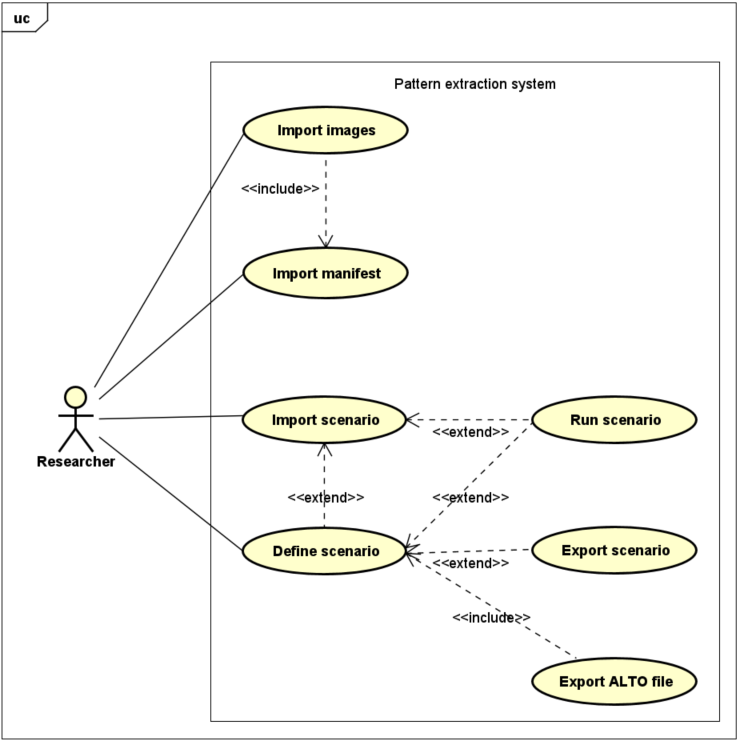
\includegraphics[width=0.6\textwidth]{pic/20221116DiagUseCase.png} 
    \caption{Use cases diagram}
    \label{diagUC}
\end{figure*}

blablabla....

\section{General structure of the system}

blablabla....

\begin{figure*}[ht] 
    \centering 
    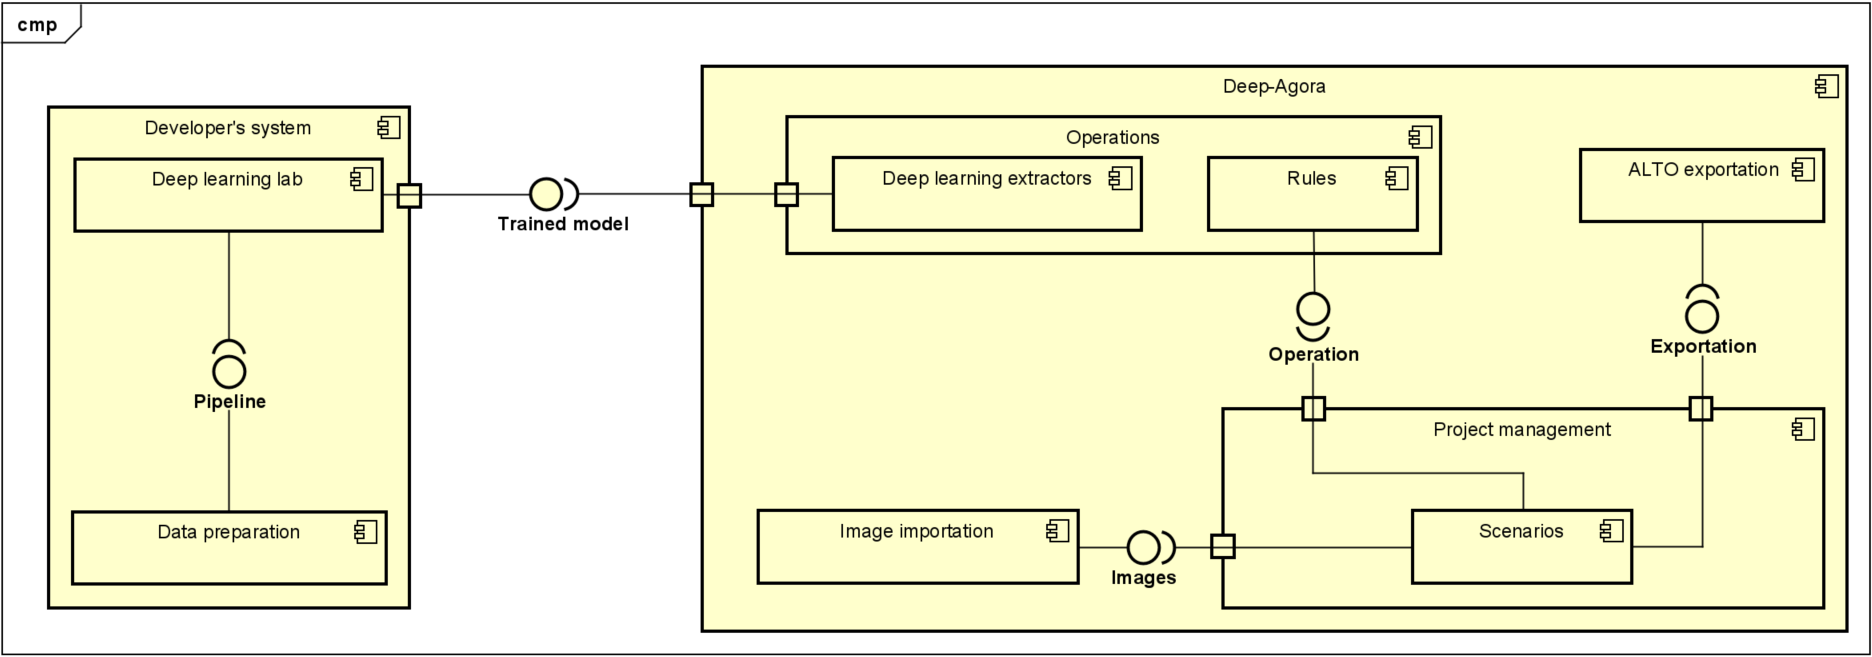
\includegraphics[width=\textwidth]{pic/20221116DiagComponent.png} 
    \caption{Component diagram}
    \label{diagComp}
\end{figure*}

blablabla....

\chapter{State of the art / Technology watch}

Sujet a définir en concertation avec votre encadrant Polytech

\section{Section 1}

PENSEZ à bien insérer TOUTES les références bibliographiques
utilisées dans votre bibliographie.

Voici un exemple de citation: \cite{DBLP:journals/corr/abs-1804-02767}.
Et une autre: \linebreak \cite{DBLP:journals/corr/RedmonDGF15}.

\paragraph{Paragraph 1}

blablabla

\begin{figure*}[ht] 
    \centering 
    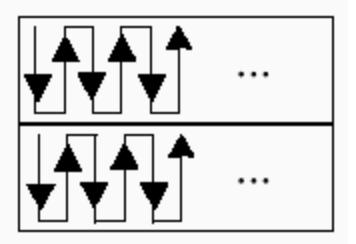
\includegraphics[width=0.5\textwidth]{pic/barre.png} 
    \caption{Fouille de données et visualisation} 
    \label{fdv} 
\end{figure*}

\paragraph{Paragraph 2}

blablabla

\section{Section 2}

blablabla


\chapter{Analysis and design}

\section{Analysis}

\subsection{Assumptions used}
blablabla

\subsection{Specifications}
Inclure ici un résumé du cahier de spécification qui sera inséré en ANNEXE

\section{Proposed modelling}

Inclure ici une description du système à développer
pouvant notamment inclure les principaux diagrammes UML non détaillés
et démontrant sa faisabilité durant la phase de mise en œuvre.

Les modes de validation prévus pour les différents éléments à produire
pourront être précisés ici.

\chapter{Implementation}

Description de vos productions et de leurs modes de réalisation.

(résumé du cahier de développement inséré en ANNEXE)

blablabla

\section{Tools and library used}

blablabla

\section{Implementation elements, technical choices}

\begin{lstlisting}[language=C++]
#include <iostream>
using namespace std;

int main () {
    cout << "Hello, world !";
    return 0;
}
\end{lstlisting}

Un exemple de PHP:
\begin{lstlisting}[language=php]
class pdfOrder extends FPDF
{
 function _check($x,$y,$width,$checked) {
   if ($checked)
     $this->rect($x,$y,$width,$width,'F');
   else
     $this->rect($x,$y,$width,$width);
 }
 function LI($sansFrais = false) {
   $LI = 'LI';
   $coord = 'Laboratoire informatique
64, avenue Jean Portalis
37200 Tours
Tél. : 02 47 36 14 42
Fax. : 02 47 36 14 22';
   $this->Image(dirname(__FILE__)  .'/li.jpg',10,2,20);
   $this->SetFont('Times','B',20);
   $this->SetFont('Times','',9);
   $this->setXY(35,3);
   $this->Multicell(80,4,utf8_decode($coord),0,'LT');
 }
\end{lstlisting}

\section{Analysis of results, evaluation, quality}

blablabla


\section{Main HMIs}

\subsection{HMI 1}

Résumé des principaux éléments présent dans le Guide de l'utilisateur
avec d'éventuels compléments d'information sur leur mode de mise en œuvre.


\chapter{Assessment and conclusion}

\section{Semester 9 review}

Liste des taches faites, en cours, à faire
CF Planning S9 et S10 à fournir en annexe

\section{Review of semester 10}

Bilan global $\Rightarrow$ respect du cahier des charges (fait / à faire)

\section{Quality assessment}
blablabla

\section{Self-critical review}
blablabla

\begin{appendix}
\selectlanguage{english}

\chapter{Planning, project management}   

\section{Evolution of the project}

Le diagramme de Gantt Initial pour la planification de ce projet 
\img{S10Gantt.png}{Le diagramme de Gantt Final}{width=1.0\textwidth}


Le diagramme de Gantt Final de ce projet est comme Figure A.2.

\img{S10Gantt.png}{Le diagramme de Gantt Final}{width=1.0\textwidth}


\section{Job description}

\paragraph{Task 1: Speaking Heading}

\begin{itemize}
    \item Date de début: 16/09/2019
    \item Date de fin: 03/10/2019
    \item Durée: 17 jours
    \item
        Description: éléments à faire,
        liste des entrées (pré-requis)
        et sorties (livrables)s de la tache.
\end{itemize}

\paragraph{Task 2: Speaking Heading}

\begin{itemize}
    \item Date de début: 16/09/2019
    \item Date de fin: 03/10/2019
    \item Durée: 17 jours
    \item
        Description: éléments à faire,
        liste des entrées (pré-requis)
        et sorties (livrables)s de la tache.
\end{itemize}


\chapter{Description of the interfaces}

\section{Hardware/software interfaces}

blablabla

\section{Human/machine interfaces}

blablabla

\chapter{Specification}

\section{Functional specifications}

\subsection{Features to be developed}


%~ \setcounter{secnumdepth}{2}
%~ \renewcommand\thesection{\arabic{section}} 

\subsection{Definition of function 1: speaking title}

\paragraph{Presentation of function 1 :}
 
\begin{description}
    \item[Élément 1] ~ \\
        Entrée : ???? \\
        Sortie : ???? \\
        Préconditions : ???? \\
        Postconditions : ????
    \item[Élément 2] ~ \\
        Entrée : ???? \\
        Sortie : ???? \\
        Préconditions : ???? \\
        Postconditions : ????
\end{description}

\subsection{Definition of function 2: speaking title}

\paragraph{Presentation of function 2:}

\begin{itemize}
    \item Nom de la fonction : Visualisation des statistiques
    \item blablabla
    \item Primordiale
\end{itemize}

\paragraph{Description de la fonction 2 :}

blablabla


\section{Non-functional specifications}

\subsection{Development constraints and design}

blablabla

\subsection{Functional and operational constraints}

\subsubsection{Performance}
blablabla

\subsubsection{Capabilities}
blablabla

\subsubsection{Controllability}
blablabla

\subsubsection{Security}
blablabla


\chapter{Developer's Workbook}

\section{Introduction}

blablabla

\section{Architectural diagrams and UML}

blablabla

\section{Detailed descriptions of data used}

blablabla

\section{Detailed descriptions of classes, modules, achievements}

blablabla


\chapter{Installation document}

Ce document regroupe toutes les informations nécessaires
pour l’installation du projet sur les machines,
ainsi que pour sa mise en production.

\chapter{User document}

blablabla

\chapter{Tests}

Les tests  visent à garantir l'exactitude,
l'intégrité, la sécurité et les performances du logiciel. 

\section{Unit testing}

blablabla

\begin{table}[]
\definecolor{C}{HTML}{305496}
\begin{tabular}{|l|l|}\hline
\color{C} IDENTIFICATION OF COMPONENT \\\hline
Afficher toutes les missions de l'utilisateur identifié  \\\hline
\color{C} DESCRIPTION OF THE TEST (granularity, scenario, values, actions) \\\hline
Action :blablabla.\\ blablabla. \\\hline
\color{C} EXPECTED RESULTS \\\hline
Cas 1: blblablaa.\\ Cas 2: blablabla. \\\hline
\color{C} OBTAINED RESULTS \\\hline
blablabla \\\hline
\end{tabular}
\end{table}                                                                             

\section{Integration testing}

blablabla

\end{appendix}

\end{document}


